\documentclass[11pt]{article}
\title{\textbf{CS 361 Spring 2018 \\ Homework 4}}
\author{Nathaniel Murphy (njmurph3)}

\usepackage{a4wide}
\usepackage{amsfonts}
\usepackage{amsmath}
\usepackage{amsthm}
\usepackage{graphicx}

\begin{document}
\maketitle

\section*{4.1}
Assuming that the roulette wheel has slots numbered 0-36,
\[P(X=x)=\begin{cases}
	\frac{1}{37} & \text{if }0\leq x\leq 36 \\
	0 & \text{otherwise}
\end{cases}\]

\section*{4.2}
\subsection*{(a)}
\[P(X\geq2)=P(X=1)+P(X=2)=\frac{1}{13}+\frac{1}{13}=\frac{2}{13}\]
\subsection*{(b)}
\[P(X\geq10)=P(X=10)+P(X=11)=\frac{1}{13}+\frac{3}{13}=\frac{4}{13}\]
\subsection*{(c)}
\[P(X\geq Y)=P(X\geq X+1 \cap X\text{ is black})+P(X\geq X-1\cap X\text{ is red})\]
\[=P(X\geq X-1)P(X\text{ is red})\hspace{3mm}\text{because of independence}\]
\[=1\cdot P(\text{X is red})\]
\[=\frac{1}{2}\]
\subsection*{(d)}
$P(Y-X)$ can take on 2 values: $\{-1,1\}$.
\[Y-X=\begin{cases}
	(X+1)-X=1 & \text{if }X\text{ is black} \\
	(X-1)-X=-1 & \text{if }X\text{ is red}
\end{cases}\]
\clearpage
which implies
\[P(Y-X=x)=\begin{cases}
	P(X\text{ is black})=\frac{1}{2} & \text{if }x=1 \\
	P(X\text{ is red})=\frac{1}{2} & \text{if }x=-1 \\
	0 & \text{otherwise}
\end{cases}\]
\subsection*{(e)}
\[P(Y\geq 12)=P(X+1\geq12\cap X \text{ is black})+P(X-1\geq12\cap X\text{ is red})\]
\[=P(X\geq11 \cap X \text{ is black})+P(X\geq 13\cap  X\text{ is red})\]
\[=P(X\geq11)P(X\text{ is black})+0\hspace{5mm}\text{because of independence}\]
\[=\left(\frac{3}{13}\right)\left(\frac{1}{2}\right)=\frac{3}{26}\]

\section*{4.3}
Let $X$ be the random variable described in the problem. Let us define two more random variables $Y$ to be the random variable of the coin flip and $Z$ to be the random variable of the die roll. \\ \\
We will define some preliminary probabilities:
\begin{itemize}
	\item $P(X=1)=P(Y=$ heads$)=\frac{1}{2}$
	\item $P(X=2)=P(Y=$ tails $\cap$ $(Z=2\cup Z=3))$ \\
	$P(X=2)=P(Y=$ tails$)(P(Z=2)+P(Z=3))\hspace{5mm}$ because of independence \\
	$P(X=2)=\left(\frac{1}{2}\right)\left(\frac{1}{3}\right)=\frac{1}{6}$
	\item $P(X=3)=1-P(X=1)-P(X=2)=1=\frac{1}{2}-\frac{1}{6}=\frac{1}{3}$
\end{itemize}
\subsection*{(a)}
\[P(X=x)=\begin{cases}
	\frac{1}{2} & \text{if }x=1 \\
	\frac{1}{6} & \text{if }x=2 \\
	\frac{1}{3} & \text{if }x=3 \\
	0 & \text{otherwise}
\end{cases}\]
\subsection*{(b)}
\[P(X\leq x)=\begin{cases}
	0 & \text{if }x<1 \\
	\frac{1}{2} & \text{if }x=1 \\
	\frac{2}{3} & \text{if }x=2 \\
	1 & \text{if }x>2
\end{cases}\]

\section*{4.6}
\subsection*{(a)}
$S=L_1+L_2=0\Rightarrow L_1=L_2=0$ because $L_1,L_2>0$. Thus,
\[P(S=0)=P(L_1=0\cap L_2=0)\]
\[=P(L_1=0)P(L_2=0)\hspace{5mm}\text{because of independence between the decks}\]
\[=\left(\frac{\binom{30}{7}}{\binom{40}{7}}\right)\left(\frac{\binom{20}{7}}{\binom{40}{7}}\right)=(0.1092)(0.00416)=4.54\times 10^{-4}\]
\subsection*{(b)}
$D=L_1-L_2=0\Rightarrow L_1=L_2$. Thus,
\[P(D=0)=P(L_1=0\cap L_2=0)+P(L_1=1\cap L_2=1)+\ldots+P(L_1=7\cap L_2=7)\]
\[=P(L_1=0)P(L_2=0)+P(L_1=1)P(L_2=1)+\ldots+P(L_1=7)P(L_2=7)\hspace{3mm}\text{because of independence}\]
\[=\sum_{i=0}^7P(L_1=i)P(L_2=i)\]
\[=\sum_{i=0}^7\left(\frac{\binom{10}{i}\binom{30}{7-i}}{\binom{40}{7}}\right)\left(\frac{\binom{20}{i}\binom{20}{7-i}}{\binom{40}{7}}\right)\approx 0.1348\]
\subsection*{(c)}
\[P(L_1=x)=\frac{\binom{10}{x}\binom{30}{7-x}}{\binom{40}{7}}\]
which implies that
\[P(L_1=x)=\begin{cases}
	0.1092 & \text{if }x=0 \\
	0.3185 & \text{if }x=1 \\
	0.344 & \text{if }x=2 \\
	0.1764 & \text{if }x=3 \\
	0.0457 & \text{if }x=4 \\
	0.00588 & \text{if }x=5 \\
	3.379\times 10^{-4} & \text{if }x=6 \\
	6.437\times 10^{-6} & \text{if }x=7
\end{cases}\]
\subsection*{(d)}
We notice that $L_1$ may take on values $x$ such that $0\leq x\leq 5$.
\[P(L_1=x\hspace{1mm}|\hspace{1mm}L_t=5)=\frac{\binom{5}{x}\binom{25}{7-x}}{\binom{30}{7}}\]
which implies that
\[P(L_1=x\hspace{1mm}|\hspace{1mm}L_t=5)=\begin{cases}
	0.2361 & \text{if }x=0 \\
	0.435 & \text{if }x=1 \\
	0.261 & \text{if }x=2 \\
	0.0621 & \text{if }x=3 \\
	0.00565 & \text{if }x=4 \\
	1.474\times10^{-4} & \text{if }x=5
\end{cases}\]

\section*{4.7}
Alternatively, 
\[g(x)=\begin{cases}
	\text{cos}(x) & \text{if }-\frac{\pi}{2}\leq x\leq\frac{\pi}{2} \\
	0 & \text{otherwise}
\end{cases}\]
\subsection*{(a)}
We know that $\int_{-\infty}^{\infty}p(x)dx=1$, so $p(x)=cg(x)\Rightarrow\int_{-\infty}^{\infty}cg(x)dx=c\int_{-\infty}^{\infty}g(x)dx=1$ \\ \\
We know that
\[\int_{-\infty}^{\infty}g(x)dx=\int_{-\frac{\pi}{2}}^{\frac{\pi}{2}}\text{cos}(x)dx=\text{sin}(x)|_{-\frac{\pi}{2}}^{\frac{\pi}{2}}=\text{sin}(\frac{\pi}{2})-\text{sin}(-\frac{\pi}{2})=1-(-1)=2\]
It follows that
\[1=c\int_{-\infty}^{\infty}g(x)dx=c\int_{-\frac{\pi}{2}}^{\frac{\pi}{2}}\text{cos}(x)dx=2\cdot c\Rightarrow c=\frac{1}{2}\]
\[p(x)=\begin{cases}
	\frac{1}{2}\text{cos}(x) & \text{if }-\frac{\pi}{2}\leq x \leq\frac{\pi}{2} \\
	0 & \text{otherwise}
\end{cases}\]
\subsection*{(b)}
By looking at a graph, we can see that on the interval $x\in[-\frac{\pi}{2},\frac{\pi}{2}]$, cos$(x)\geq0$. Therefore, $P(X\geq0)=1$.
\subsection*{(c)}
From our knowledge of the cosine function, we know that the magnitude is never greater than 1 which implies that the magnitude of $\frac{1}{2}$cos$(x)$ can never be greater than $\frac{1}{2}$. Thus, $P(|X|\leq1)=1$.

\section*{4.9}
\subsection*{(a)}
\[\mathbb{E}[L_1]=\sum_{i=0}^7P(L_1=i)\cdot i=\sum_{i=0}^7\left(\frac{\binom{10}{i}\binom{30}{7-i}}{\binom{40}{i}}\right)\cdot i=\frac{7}{4}=1.75\]
\subsection*{(b)}
\[\mathbb{E}[L_2]=\sum_{i=0}^7P(L_2=i)\cdot i=\sum_{i=0}^7\left(\frac{\binom{20}{i}\binom{20}{7-i}}{\binom{40}{7}}\right)\cdot i=\frac{7}{2}=3.5\]
\subsection*{(c)}
var$[L_1]=\mathbb{E}[L_1^2]-\mathbb{E}[L_1]^2$.
\[\mathbb{E}[L_1^2]=\sum_{i=0}^7P(L_1=i)\cdot i^2=\sum_{i=0}^7\left(\frac{\binom{10}{i}\binom{30}{7-i}}{\binom{40}{7}}\right)\cdot i^2=\frac{217}{52}\]
\[\text{var}[L_1]=\mathbb{E}[L_1^2]-\mathbb{E}[L_1]^2=\frac{217}{52}-\left(\frac{7}{4}\right)^2=\frac{217}{52}-\frac{49}{16}=\frac{231}{208}\]

\section*{4.12}
\subsection*{(a)}
Let $X_3$ be a random variable that three people play one round.
\[P(X_3=\text{1T, 2H }\cup\hspace{1mm}X_3=\text{1H, 2T})=P(X_3=\text{1T, 2H})+P(X_3=\text{1H, 2T})\]
\[\frac{\binom{3}{1}}{2^3}+\frac{\binom{3}{1}}{2^3}=\frac{3}{8}+\frac{3}{8}=\frac{3}{4}\]
\subsection*{(b)}
Let $X_4$ be a random variable that four people play one round.
\[P(X_4=\text{1T, 3H }\cup\hspace{1mm}X_4=\text{1H, 3T})=P(X_4=\text{1T, 3H})+P(X_4=\text{1H, 3T})\]
\[\frac{\binom{4}{1}}{2^4}+\frac{\binom{4}{1}}{2^4}=\frac{4}{16}+\frac{4}{16}=\frac{1}{2}\]
\subsection*{(c)}
Let $X_5$ be a random variable that five people play one round.
\[P(X_5=\text{1T, 4H }\cup\hspace{1mm}X_5=\text{1H, 4T})=P(X_5=\text{1T, 4H})+P(X_5=\text{1H, 4T})\]
\[\frac{\binom{5}{1}}{2^5}+\frac{\binom{5}{1}}{2^5}=\frac{5}{16}\]
Let $Y_5$ be the number of rounds are played until there is an odd person out.
\[P(Y_5=x)=\left(\frac{11}{16}\right)^{x-1}\left(\frac{5}{16}\right)\]
\[\mathbb{E}[Y_5]=\left(\frac{5}{16}\right)^{-1}=\textbf{3.2}\text{ \textbf{rounds} (Expectation of Bernoulli)}\]

\section*{4.14}
Let us assume that $X$ and $Y$ are independent random variables.
\[\text{var}[X+Y]=\mathbb{E}[(X+Y)^2]-\mathbb{E}[X+Y]^2\]
\[=\mathbb{E}[X^2+2XY+Y^2]-\left(\mathbb{E}[X]+\mathbb{E}[Y]\right)^2\]
\[=\mathbb{E}[X^2]+2\mathbb{E}[XY]+\mathbb{E}[Y^2]-\mathbb{E}[X]^2-2\mathbb{E}[X]\mathbb{E}[Y]-\mathbb{E}[Y]^2\]
\[=\mathbb{E}[X^2]+2\mathbb{E}[X]\mathbb{E}[Y]+\mathbb{E}[Y^2]-\mathbb{E}[X]^2-2\mathbb{E}[X]\mathbb{E}[Y]-\mathbb{E}[Y]^2\]
\[=\left(\mathbb{E}[X^2]-\mathbb{E}[X]^2\right)+\left(\mathbb{E}[Y^2]-\mathbb{E}[Y]^2\right)\]
\[=\text{var}[X]+\text{var}[Y]\]
\qed

\section*{4.16}
We know that $\mathbb{E}[|X|]=0.2$ and $P(|X|=0)=P(X=0)$.
\[P(X=0)=1-\big(P(|X|=1)+P(|X|+2)\big)=1-P(|X|\geq1)\]
Finding an upper bound for $P(|X|\geq1)$ will find a lower bound for $1-P(|X|\geq1)$.
\[P(|X|\geq1)\leq\frac{\mathbb{E}[|X|]}{1}\]
\[P(|X|\geq1)\leq0.2\]
It follows that a lower bound for $P(X=0)=1-P(|X|\geq1)=1-0.2=0.8$

\section*{4.17}
\[\mathbb{E}[X]=2\Rightarrow P(X=2)=1-P(|X-\mathbb{E}[X]|>0)\]
and, since $X$ is a discrete random variable,
\[1-P(|X-\mathbb{E}[X]|>0)=1-P(|X-\mathbb{E}[X]|\geq1)\]
We clearly see that finding an upper bound for $P(|X-\mathbb{E}[X]|\geq1)$ will result in a lower bound for $1-P(|X-\mathbb{E}[X]|\geq1)$. Using Chebyshev's inequality,
\[P(|X-\mathbb{E}[X]|\geq1)\leq\frac{\text{var}[X]}{1}\]
\[P(|X-\mathbb{E}[X]|\geq1)\leq0.01\]
It follows that
\[1-P(|X-\mathbb{E}[X]|\geq1)=1-0.01=0.99\Rightarrow P(X=2)\geq 0.99\]

\section*{4.22}
\subsection*{(a)}
Let $X$ be a rondom variable for the number of passengers that show up to the flight.
\[\mathbb{E}[X]=\sum_{i=0}^6P(X=x)\cdot i=\sum_{i=0}^6\binom{6}{i}\left(p^i(1-p)^{6-i}\right)\cdot i=\sum_{i=0}^6\binom{6}{i}\big((0.9)^i(0.1)^{6-i}\big)\cdot i=5.4\]
\subsection*{(b)}
We want $\mathbb{E}[X]\geq 6$. The following program simulates $\mathbb{E}[X]$ given that $n$ tickets are sold. Wee see that the smallest value of $n$ to give an expectation less than 6 is $n=10$ tickets.
\begin{figure}[h!]
	\centering
	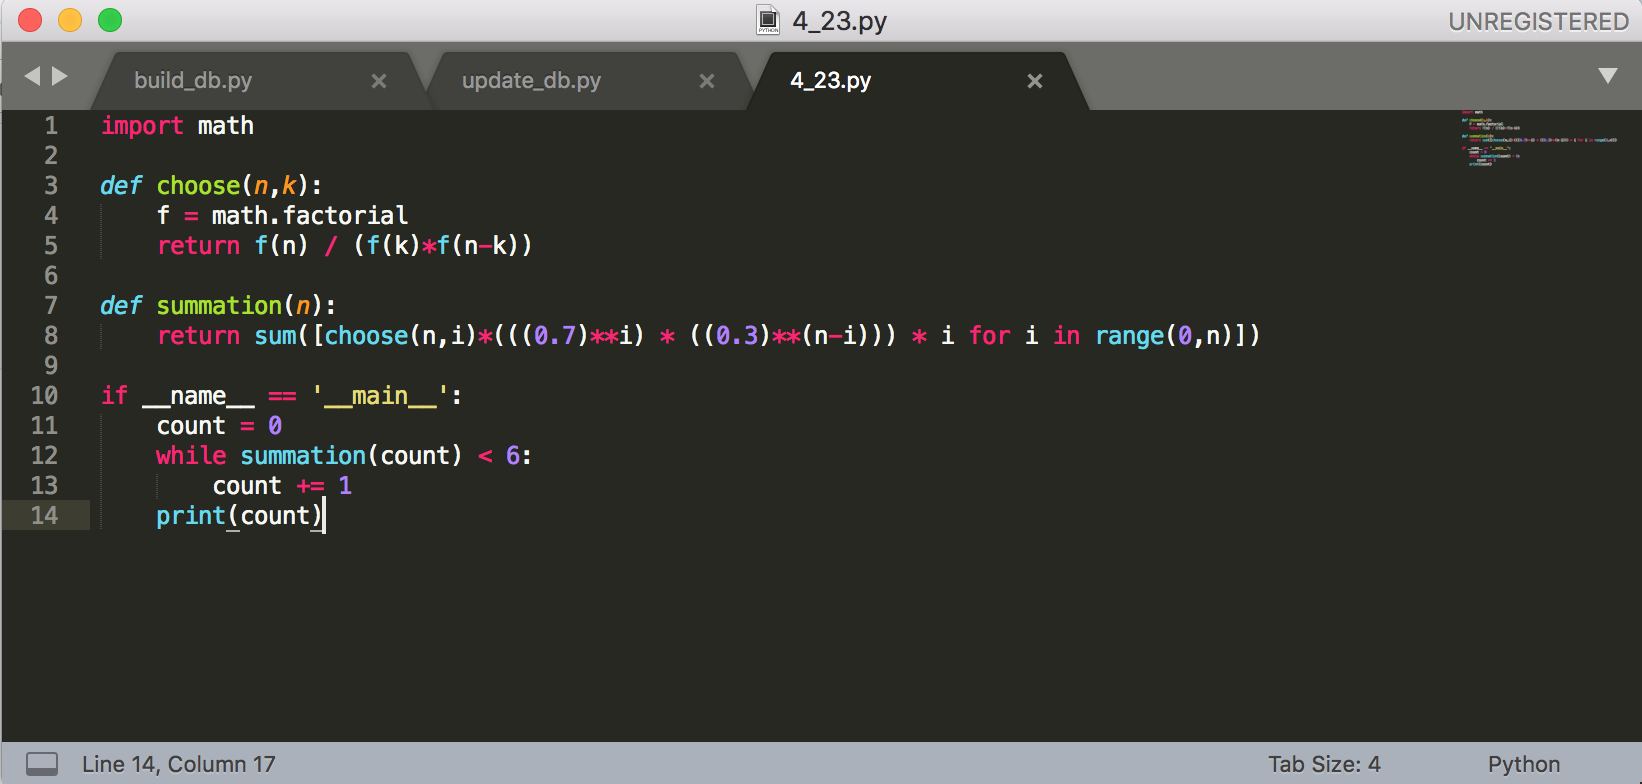
\includegraphics[width=\textwidth]{4_22.png}
\end{figure}

\section*{4.23}
\subsection*{(a)}
Let $X$ be the random variable that represents how many passengers show up to their flight. Let $n$ represent the number of tickets sold.
\[P(X=x)=\begin{cases}
	\binom{n}{x}p^x(1-p)^{n-x} & \text{if }0\leq x\leq n \\
	0 & \text{otherwise}
\end{cases}\]
We see that random variable $X$ follows a binomial distribution, and thus, we know that $\mathbb{E}[X]=np$, where $p$ is the probability of a pasenger showing upt to his/her flight. We want
\[\mathbb{E}[X]=np\geq10\]
It follows that when $n\geq\frac{10}{p}$ tickets are sold, the expected number of passengers that show up is greater than 10.
\subsection*{(b)}
Upon running the following simulation with various values of $p$, I found that
\[\mathbb{E}[(X\hspace{1mm}|\hspace{1mm}\text{flight takes off})]=10\cdot p\]
Which follows from the event that someone shows up to their flight and the event that the passenger is a woman are independent events.
\begin{figure}[h!]
	\centering
	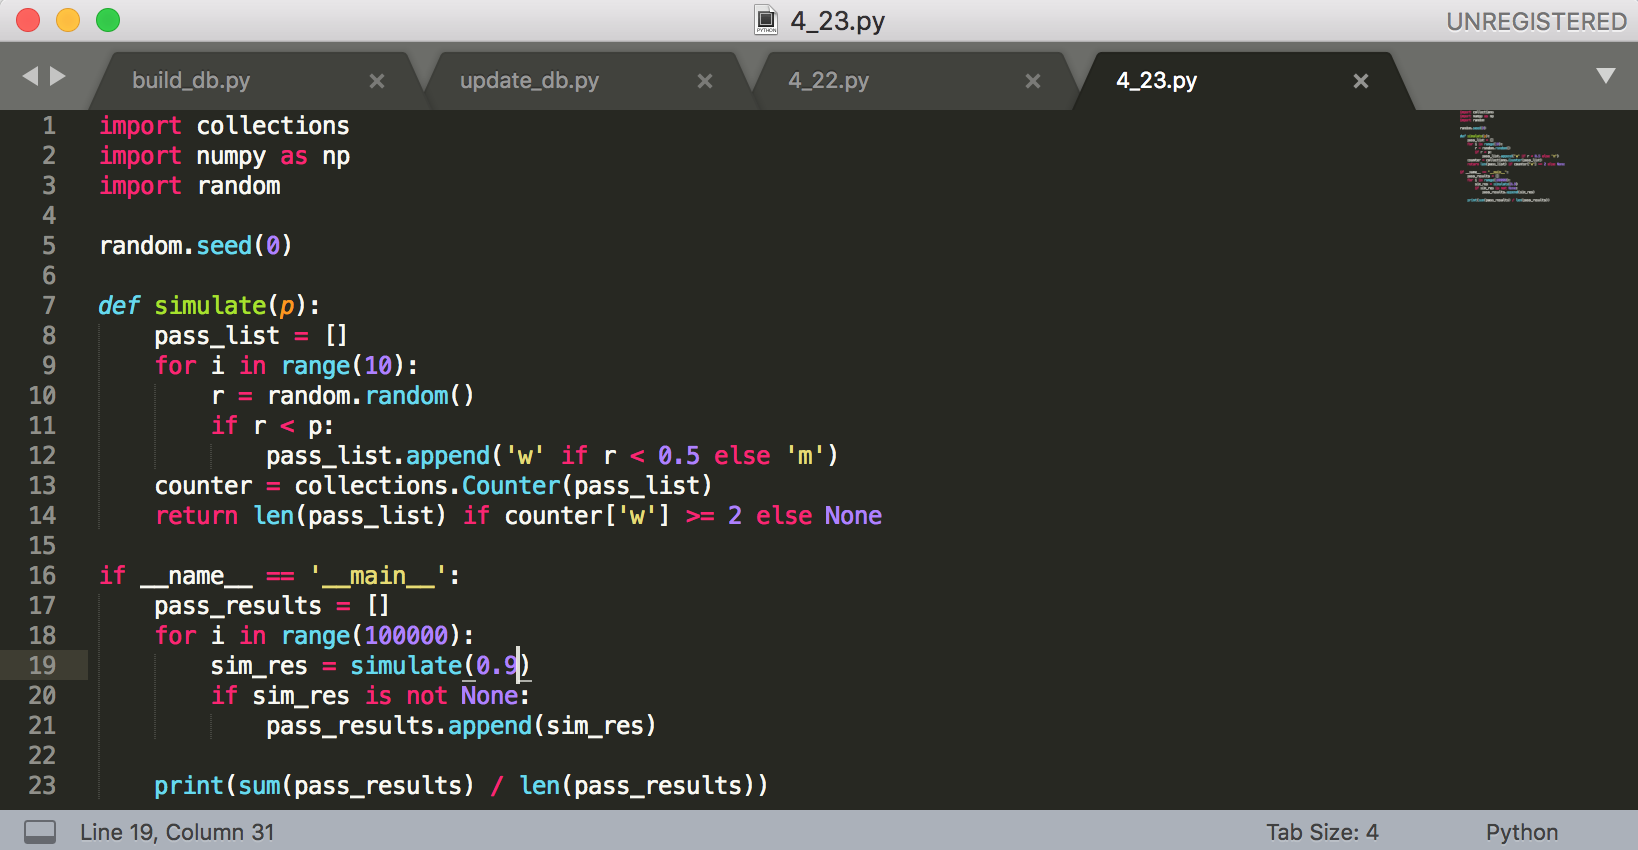
\includegraphics[width=\textwidth]{4_23.png}
\end{figure}
\end{document}